\chapter{Resultados e Discussão}
\label{cap:resultados}

Este capítulo apresenta e discute os principais resultados obtidos ao longo do desenvolvimento do sistema automatizado de limpeza e manutenção de piscinas. São analisados o desempenho operacional da solução proposta, os desafios técnicos enfrentados durante a implementação e as estratégias adotadas para mitigá-los. A discussão contempla a integração do protótipo físico, a usabilidade da interface de controle desenvolvida e a confiabilidade dos dados coletados, destacando os avanços alcançados em relação aos métodos manuais tradicionais, bem como as limitações observadas no contexto experimental.

\section{Integração do Protótipo Físico}

O desenvolvimento do protótipo físico possibilitou a consolidação da arquitetura definida na fase de Elaboração, permitindo validar, de forma prática, a integração entre sensores, atuadores e a central de controle. O conjunto foi acondicionado em uma caixa de papelão coberta por uma placa de isopor com o objetivo de simular um ambiente real de operação e prover proteção básica aos componentes eletrônicos contra respingos e umidade, características inerentes ao contexto de uso em piscinas.

A disposição dos sensores de pH, turbidez, temperatura e nível no reservatório de testes mostrou-se adequada para a realização de leituras contínuas, contribuindo para a obtenção de dados consistentes ao longo dos experimentos. Essa configuração evidenciou boa confiabilidade na coleta das variáveis monitoradas, aspecto essencial para o funcionamento correto do ciclo de automação proposto.

A Figura \ref{fig:prototipo_final} apresenta uma visão geral do protótipo montado, destacando a interligação entre a central de controle e os dispositivos responsáveis pela medição e atuação no sistema.

\begin{figure}[H]
    \centering
    \caption{Protótipo final do sistema de automação montado.}
    \label{fig:prototipo_final}
    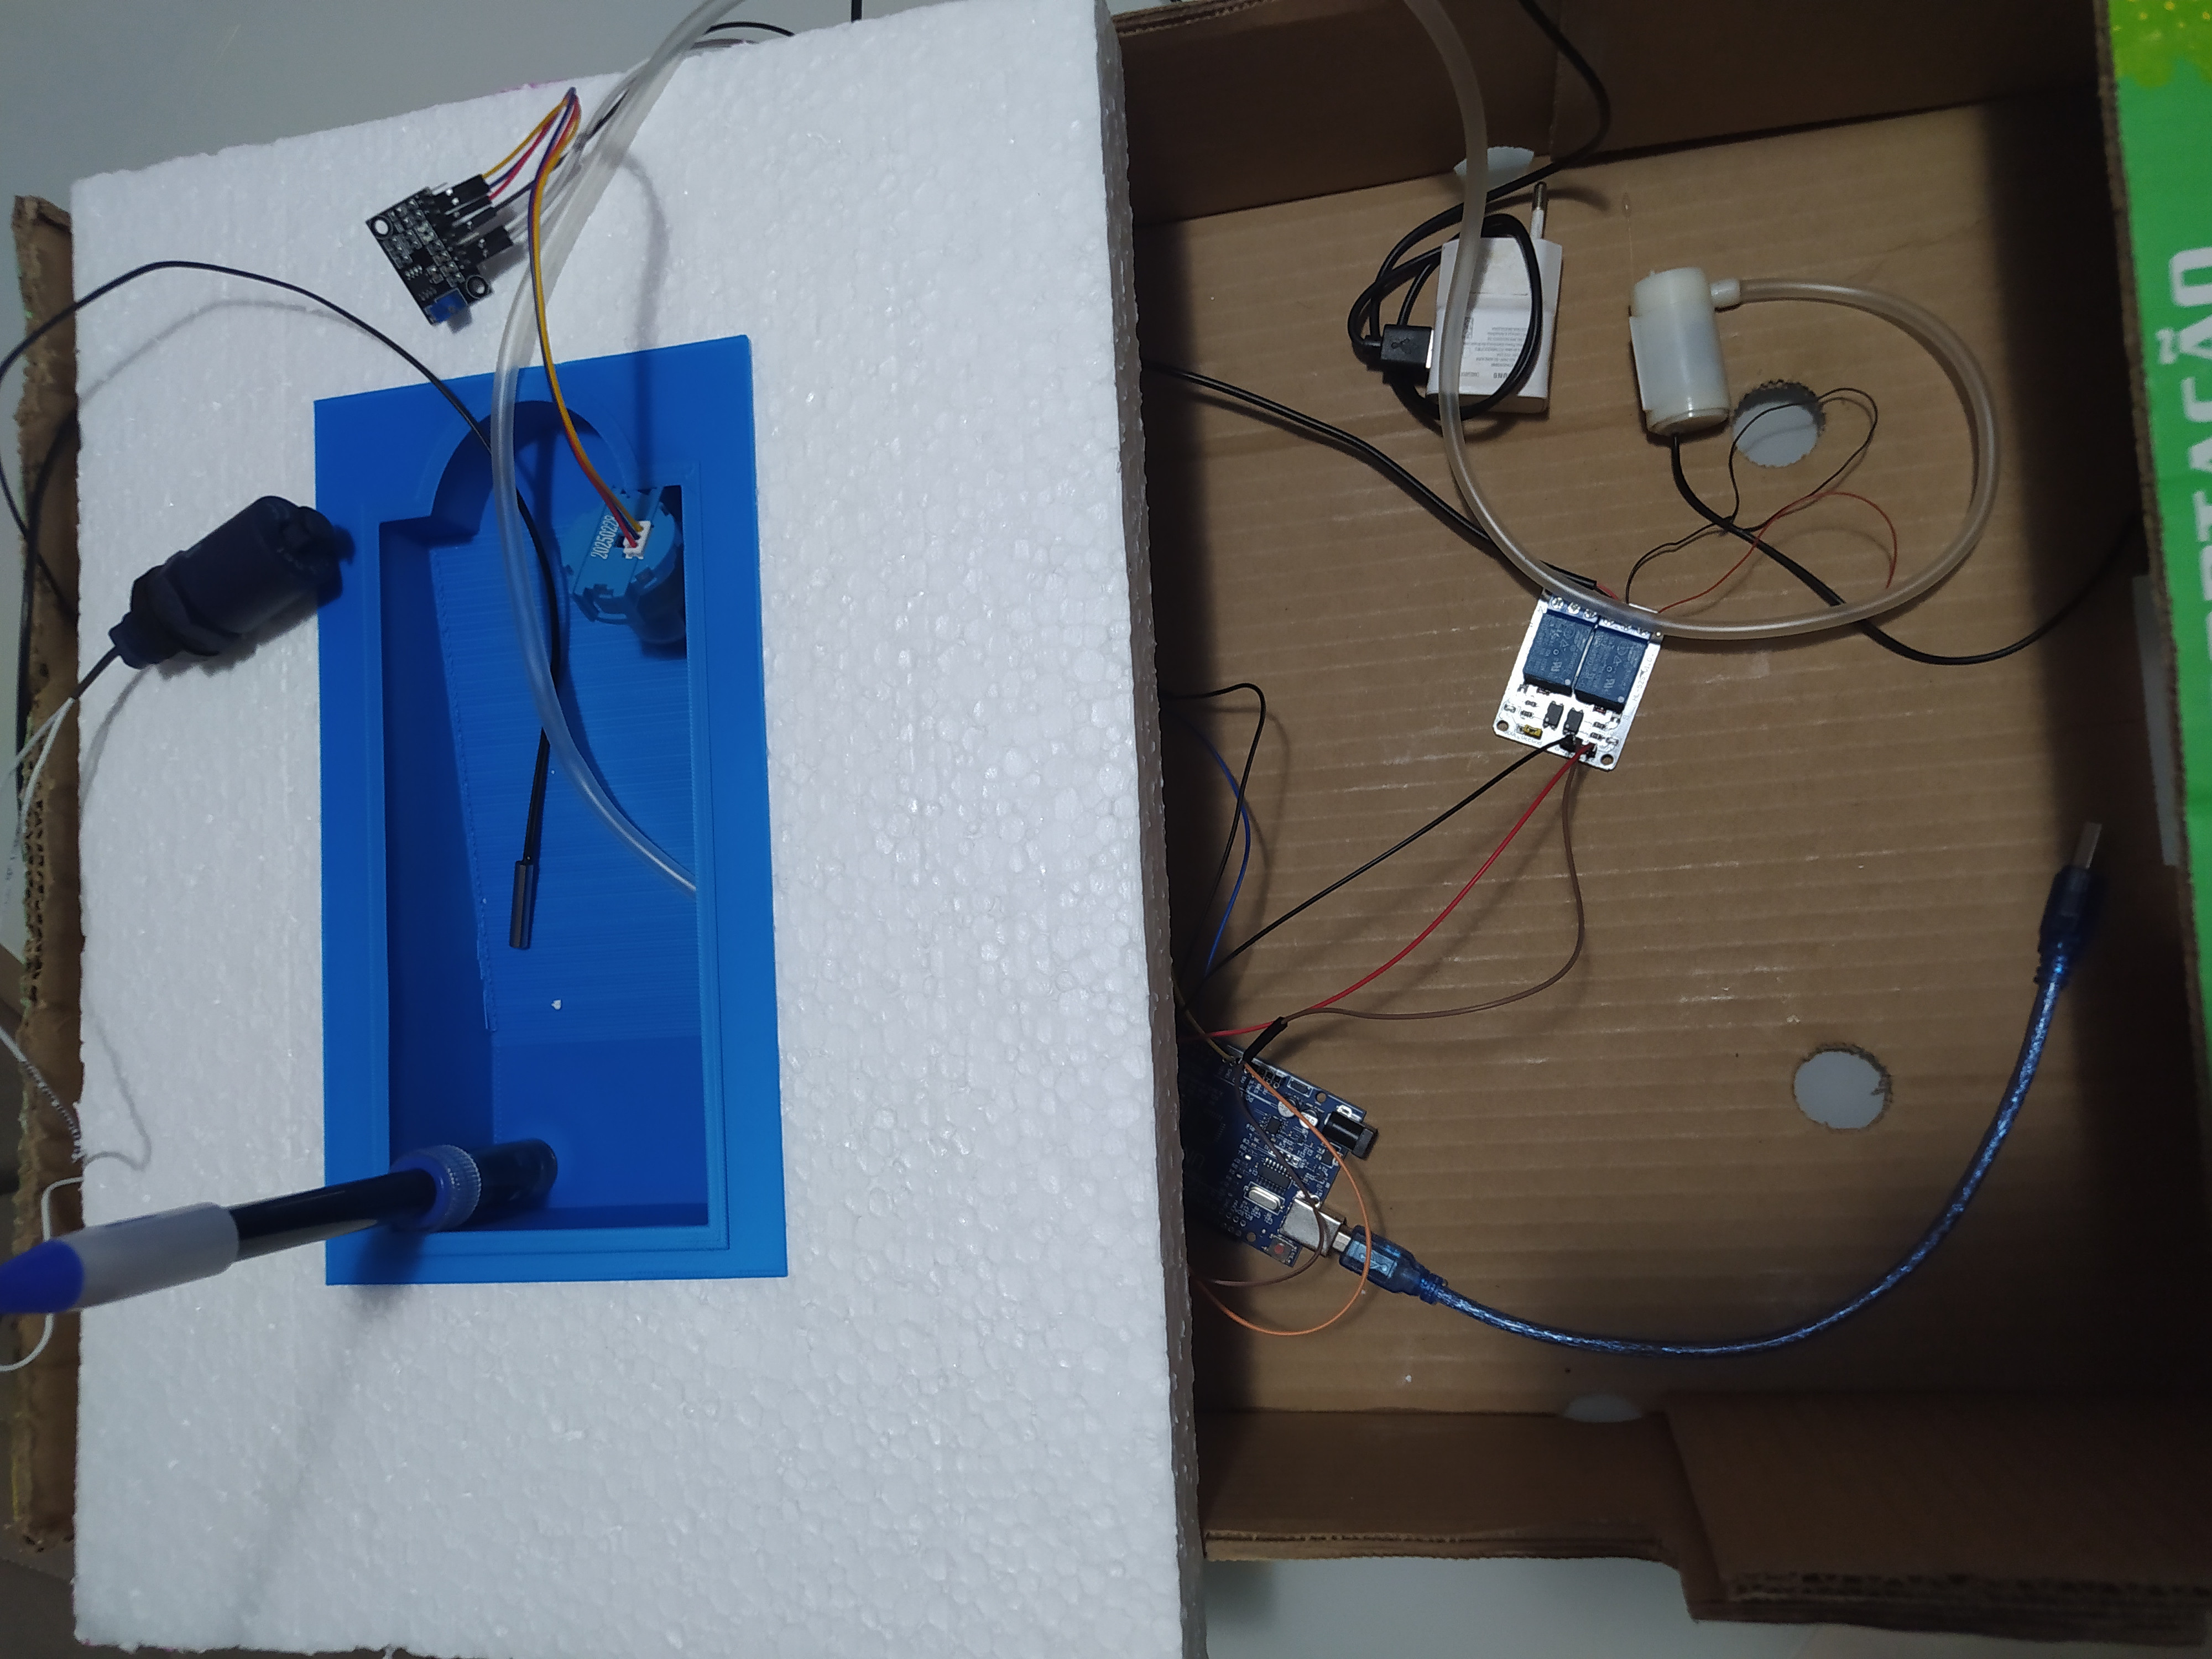
\includegraphics[width=0.8\textwidth]{imagens/prototipoFinal.jpg}
    \caption*{Fonte: Autoria própria (2025).}
\end{figure}

Durante os testes de integração, o conjunto de atuadores apresentou comportamento compatível com o esperado, com o acionamento da bomba d’água por meio do relé ocorrendo de forma quase imediata. Entretanto, nas etapas iniciais de validação, foi identificado um problema relacionado à estabilidade do sistema: o acionamento da bomba gerava ruídos eletromagnéticos e picos de tensão que interferiam no funcionamento do microcontrolador, comprometendo tanto a estabilidade das leituras dos sensores quanto a operação contínua do atuador.

Para mitigar esse problema, optou-se pela substituição do módulo de acionamento simples por um módulo relé com isolamento por optoacoplador. Essa solução proporcionou o isolamento galvânico entre o circuito de potência e o circuito lógico do Arduino, eliminando as interferências previamente observadas e aumentando a robustez do sistema. A Figura \ref{fig:rele_opto} apresenta o componente adotado após essa modificação.

\begin{figure}[H]
    \centering
    \caption{Relé com optoacoplador.}
    \label{fig:rele_opto}
    \includegraphics[width=0.60\textwidth]{imagens/releFinal.jpeg}
    \caption*{Fonte: Autoria própria (2025).}
\end{figure}

Além das questões relacionadas ao acionamento dos atuadores, foram identificadas limitações associadas à calibração inicial de alguns sensores. O sensor de pH, por exemplo, apresentou descalibração de fábrica, exigindo ajuste manual no módulo ao qual estava acoplado. A calibração foi realizada em nível de \textit{hardware}, por meio do ajuste do potenciômetro (\textit{trimpot}) de \textit{offset} da placa condicionadora, alinhando a tensão de saída ao valor de referência esperado.

O procedimento de calibração foi validado utilizando-se uma garrafa de água mineral lacrada, cujo pH declarado é de 6,98. Após o ajuste, o sensor apresentou leituras variando entre 6,78 e 6,80, valor considerado satisfatório para o contexto experimental, conforme ilustrado na Figura \ref{fig:sensorpH:sendoCalibrado}.

\begin{figure}[H]
    \centering
    \caption{Validação do sensor de pH.}
    \label{fig:sensorpH:sendoCalibrado}
    \includegraphics[width=1.00\textwidth]{imagens/calibracaoSensorPh.png}
    \caption*{Fonte: Autoria própria (2025).}
\end{figure}

De forma semelhante, o sensor de temperatura apresentou desvios iniciais em relação ao valor real da água. A correção foi realizada via \textit{software}, por meio da aplicação de um fator de ajuste na equação do divisor de tensão, compensando variações na resistência nominal do termistor do tipo NTC. A validação do ajuste foi conduzida com base na comparação entre a leitura fornecida por um termômetro de piscina e os valores obtidos pelo sensor, registrando-se 25,7~°C no instrumento de referência e 25,93~°C no sistema desenvolvido. Essa proximidade entre os valores confirma a adequação do processo de calibração, conforme apresentado na Figura \ref{fig:sensorTemperatura:sendoCalibrado}.

\begin{figure}[H]
    \centering
    \caption{Validação do sensor de temperatura.}
    \label{fig:sensorTemperatura:sendoCalibrado}
    \includegraphics[width=1.00\textwidth]{imagens/calibrandoSesorTemperatura.png}
    \caption*{Fonte: Autoria própria (2025).}
\end{figure}

\section{Interface de Controle e Monitoramento}

A interface de controle desenvolvida para o sistema, implementada no \textit{front-end} com a biblioteca React, foi projetada com o objetivo de centralizar informações técnicas complexas em um \textit{dashboard} visualmente intuitivo. Essa abordagem busca abstrair a complexidade inerente aos sensores e ao processamento dos dados, permitindo que o usuário compreenda rapidamente o estado da piscina sem a necessidade de conhecimentos técnicos avançados.

Diferentemente de soluções que exigem interpretação direta de valores brutos ou interação por meio de \textit{displays LCD} acoplados ao hardware, a interface web apresenta os principais indicadores de qualidade da água de forma gráfica e organizada. Ao acessar o sistema, o usuário visualiza, em tempo real, os cartões de status referentes aos parâmetros monitorados, como pH, temperatura, turbidez e estado da bomba.

A comunicação entre o \textit{front-end} e o \textit{back-end}, desenvolvido em Spring Boot, garante a atualização periódica dos dados exibidos, permitindo o acompanhamento contínuo da evolução do tratamento da água. Além do monitoramento passivo, a interface oferece recursos de controle ativo, possibilitando ao usuário ligar ou desligar manualmente o sistema de filtragem. Essa funcionalidade permite a sobreposição temporária da lógica de automação em situações específicas, como manutenções corretivas ou testes operacionais.

A Figura \ref{fig:dashboard_web} apresenta a tela principal do sistema, evidenciando a disposição dos indicadores e o foco na clareza das informações exibidas.

\begin{figure}[H]
    \centering
    \caption{Interface Web: Dashboard de monitoramento em tempo real.}
    \label{fig:dashboard_web}
    \includegraphics[width=1.0\textwidth]{imagens/printSistema.png}
    \caption*{Fonte: Autoria própria (2025).}
\end{figure}

\vspace{5em}

\section{Análise de Desempenho e Discussão}

Os testes práticos realizados no cenário de validação demonstraram que o sistema é capaz de executar de forma consistente o ciclo completo de automação proposto, abrangendo as etapas de leitura dos sensores, processamento dos dados, transmissão das informações e atuação sobre os dispositivos físicos. Essa integração confirmou a viabilidade da arquitetura adotada para aplicações de automação residencial em piscinas.

No que se refere à precisão das medições, o sensor de temperatura NTC 10K apresentou elevada estabilidade, com variações consideradas desprezíveis quando comparadas às leituras obtidas por meio de um termômetro de referência. Esse comportamento evidencia a adequação do componente para monitoramento térmico contínuo em ambientes domésticos. Em contrapartida, os sensores analógicos voltados à avaliação da qualidade da água demandaram um tratamento mais cuidadoso, tanto em nível de \textit{hardware} quanto de \textit{software}.

Durante os testes iniciais, observou-se que, na ausência de técnicas de filtragem digital, as leituras de pH e turbidez apresentavam oscilações momentâneas decorrentes de ruídos elétricos e variações ambientais. Essas flutuações poderiam ocasionar acionamentos indevidos da bomba, comprometendo a eficiência do sistema e aumentando o desgaste dos componentes. Para mitigar esse comportamento, foram implementados filtros de média móvel no \textit{firmware} do Arduino, estratégia que reduziu significativamente o ruído nas leituras e proporcionou maior estabilidade ao processo decisório. Após essa intervenção, o sistema apresentou desempenho compatível com os requisitos de uso doméstico, mantendo respostas coerentes com as condições reais da água.

Outro aspecto relevante avaliado foi a latência de comunicação, definida como um dos requisitos não funcionais críticos do sistema. Os experimentos indicaram que o tempo médio entre a detecção de um evento físico (como a identificação de nível inadequado de água) e a atualização correspondente na interface web permaneceu, na maioria dos testes, abaixo de cinco segundos. Esse resultado valida a eficiência da arquitetura distribuída baseada em API REST e demonstra que a solução atende às demandas típicas de aplicações IoT residenciais, nas quais a resposta em tempo quase real é suficiente para garantir segurança e confiabilidade operacional.

Apesar dos resultados positivos, algumas limitações foram identificadas. Destacam-se a sensibilidade dos sensores analógicos de baixo custo, mais suscetíveis a ruídos e variações ambientais, e a dependência da estabilidade da rede Wi-Fi local, fator que pode impactar a atualização contínua da interface em cenários com conectividade limitada. Tais restrições não comprometem a funcionalidade do protótipo, mas indicam a necessidade de aprimoramentos para aplicações em maior escala ou ambientes com exigências mais rigorosas. Esses aspectos orientam as propostas de evolução do sistema, discutidas na seção de trabalhos futuros.

\section{Trabalhos futuros}

Como continuidade deste trabalho, diversas possibilidades de aprimoramento podem ser exploradas a fim de ampliar a robustez, a autonomia e a escalabilidade do sistema desenvolvido. Uma evolução natural consiste na integração de um sensor de cloro livre, baseado em potencial de oxirredução (ORP), permitindo completar o ciclo de automação química da piscina e oferecer um controle mais preciso da desinfecção da água.

Outra linha promissora refere-se à aplicação de algoritmos de aprendizado de máquina voltados à manutenção preditiva. A partir do histórico operacional armazenado no sistema, seria possível identificar padrões de funcionamento e antecipar falhas em bombas, sensores ou outros componentes, reduzindo custos de manutenção e aumentando a confiabilidade da solução ao longo do tempo.

Adicionalmente, recomenda-se a implementação do sistema em piscinas de alvenaria em escala real, possibilitando a avaliação do desempenho em condições mais próximas do uso cotidiano. Esse cenário permitiria analisar o comportamento do sistema sob diferentes volumes de água, condições ambientais e perfis de utilização, contribuindo para a validação de sua aplicabilidade prática e para eventuais ajustes de projeto.

No que diz respeito à escalabilidade, futuras versões do sistema podem incorporar suporte a múltiplas piscinas e usuários simultâneos, ampliando seu escopo de aplicação para condomínios, clubes ou empreendimentos de lazer. Para sustentar essa expansão, propõe-se a adoção de uma arquitetura orientada a eventos no \textit{back-end}, utilizando o padrão de projeto \textit{Observer}. Essa abordagem permitiria que a interface web fosse notificada de forma proativa e praticamente instantânea sempre que novas leituras fossem processadas, eliminando a necessidade de requisições cíclicas (\textit{polling})\footnote{Técnica na qual um sistema realiza verificações periódicas em intervalos regulares para identificar a ocorrência de novos dados ou eventos.}. Como resultado, espera-se uma redução no consumo de recursos computacionais, maior eficiência na comunicação e uma experiência de uso mais fluida para o usuário final.


    